Os SIA são sistemas adaptativos inspirados pela imunologia teórica e pelas funções imunológicas observadas, princípios e modelos, que são aplicados à resolução de problemas. Eles são tipicamente modelados após as caracteristicas de aprendizado e memória do sistema imunológico para uso na resolução de problemas \cite{boccato2024}. Os principais modelos de SIA incluem algoritmos de seleção clonal e negativa, e modelos de rede.

\section{Seleção clonal e negativa}
\thispagestyle{mystyle}

A seleção clonal e negativa são dois mecanismos fundamentais do sistema imunológico que foram adaptados para uso em SIA.

\begin{figure}[h]
\centering
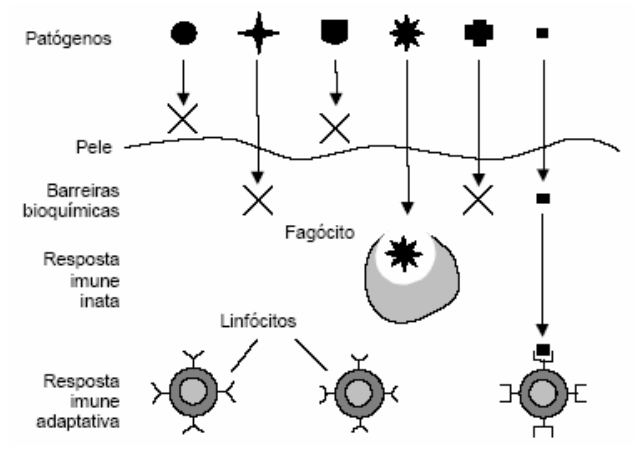
\includegraphics[width=0.5\textwidth]{imgs/camadas_defesa_sistema_imunologico.png}
\caption{Camadas de defesa do sistema imunológico.}
\label{fig:selecao_clonal_negativa}
Fonte: \cite{castro1999}
\end{figure}

A \textbf{seleção clonal} é um processo pelo qual as células imunológicas (linfócitos B\footnote{Os \textbf{linfócitos} são um tipo de leucócito ou glóbulo branco do sangue, responsáveis pelo reconhecimento e destruição de micro-organismos infecciosos como bactérias e vírus \cite{todamateria2024}. Os \textbf{linfócitos B} são os responsáveis por garantir a chamada imunidade humoral, que se destaca pela resposta imunológica realizada pela produção de anticorpos. Esses anticorpos são capazes de neutralizar ou ainda destruir os antígenos\cite{santos2024linfocitos}. }) que reconhecem um antígeno\footnote{Os \textbf{antígenos} podem ser definidos como moléculas que podem ligar-se aos anticorpos. Muitos autores preferem defini-lo como qualquer substância capaz de promover uma resposta por parte do sistema imunológico, entretanto, existem substâncias antigênicas que reagem com o anticorpo, mas não são capazes de estimular sua produção. Fonte: \cite{santos2024antigenos}} são selecionadas para proliferação e diferenciação. Este processo é usado para aumentar o número de células que podem reconhecer e responder a um antígeno específico \cite{williams2024}

A \textbf{seleção negativa} é um mecanismo pelo qual as células imunológicas que reagem fortemente aos próprios antígenos do corpo são eliminados, ajudando a prevenir respostas imunológicas prejudiciais ao próprio corpo \cite{greensmith2022}. Em SIA, a seleção negativa é usada para detectar anomalias ou padrões desconhecidos, fornecendo uma forma de detecção de novidade \cite{williams2024}.

\section{Modelos de rede}
\thispagestyle{mystyle}

Os modelos de rede em SIA são inspirados pela forma como as células imunológicas interagem entre si para coordenar respostas imunológicas. Estes modelos podem ser usados para resolver uma variedade de problemas, incluindo detecção de anomalias, otimização e reconhecimento de padrões \cite{greensmith2022}.

Um exemplo de um modelo de rede em SIA é a abordagem de \textbf{rede idiotípica}\footnote{A \textbf{rede idiotípica} é um conceito na imunologia que se refere a uma rede de interações entre diferentes tipos de células imunológicas \cite{Lemke2005}.}, que modela as interações complexas entre diferentes tipos de células imunológicas. Este modelo pode ser usado para criar sistemas que são capazes de aprendizado e memória, permitindo que eles se adaptem a novos desafios ao longo do tempo \cite{greensmith2022}.

Outro exemplo é o \textbf{Algoritmo de Células Dendríticas}, que modelo o papel das células dendríticas\footnote{As \textbf{células dendríticas} são leucócitos originários da medula óssea, presentes no sangue, pele e sistemas digestivo e respiratório. Elas identificam infecções e desencadeiam a resposta imune \cite{tuasaude2022}.} no sistema imunológico. Este algoritmo pode ser usado para detectar anomalias em dados complexos\footnote{Os tipos de dados compostos, também conhecidos como tipos de \textbf{dados complexos}, são um conjunto de tipos de dados que podem armazenar um valor de cada vez \cite{cursa2024}.} e ruidosos\footnote{\textbf{\textit{Noisy data}}, ou \textbf{dados ruidosos}, podem ser causados por uma variedade de fatores, incluindo coleta inadequada de dados, erros humanos, falhas nos sistemas de coleta e problemas durante a transmissão dos dados \cite{maiconramos2024}}, tornando-o útil para aplicações como detecção de invasões em sistemas de computador \cite{greensmith2022}.

\chapter{\MakeUppercase{Algoritmo de Seleção Negativa}}
\thispagestyle{mystyle}

O Algoritmo de Seleção Negativa se baseia no processo do sistema imunológico que envolve a \textbf{maturação}\footnote{A \textbf{maturação celular} é um processo biológico fundamental para o desenvolvimento e manutenção dos organismos vivos. Envolve uma série de etapas complexas, incluindo a proliferação, diferenciação e especialização das células \cite{cisce2024}.} das células-T, também conhecidas como \textbf{linfócitos-T}\footnote{\textbf{Linfócitos-T} são células do sistema imunológico responsáveis pela defesa do organismo contra agentes desconhecidos(antígenos) \cite{maestrovirtuale2024}.}, tornando-as capazes de identificar os \textbf{não-próprios}\footnote{\textbf{Não-próprios} se refere a elementos que não são próprios, ou seja, que são estranhos ou não pertencem ao sistema \cite{microbiologybook2024}.}. No âmbito do algoritmo, \textbf{hiperesferas}\footnote{\textbf{Hiperesferas} são uma generalização da esfera para um espaço euclidiano de dimensão arbitrária \cite{weisstein2024}} são empregadas para representar os detectores em um espaço de dados \textbf{N-dimensional}\footnote{Dados \textbf{N-dimensional} se referem a dados que existem em um espaço de N dimensões \cite{ndimensional2022}} \cite{aispackage2024}.

\section{Como o Algoritmo de Seleção Negativa é usado nos SIA}
\thispagestyle{mystyle}

Nos Sistemas Imunológicos Artificiais (SIA), o Algoritmo de Seleção Negativa é usado para identificar anomalias ou intrusões. Ele gera um conjunto de detectores que não correspondem a nenhum padrão normal (próprio). Esses detectores podem então identificar qualquer entrada que não seja considerada normal (não-próprio).

\subsection{Aplicações e exemplos do Algoritmo de Seleção Negativa}

\begin{itemize}
    \item \textbf{Detecção de arritmias cardiacas}: O Algoritmo de Seleção Negativa foi aplicado para detectar arritmias cardíacas em sinais de eletrocardiogramas (ECGs). Os resultados mostraram uma sensibilidade de 81,96\% e uma especificidade de 62,41\%, indicando que o algoritmo tem potencial para ser explorado por pesquisadores \cite{petrikicz2016}.

    \item \textbf{Detecção de spams}: O algoritmo também foi implementado para a detecção de spams em e-mails. A aplicação foi capaz de identificar se uma mensagem de e-mail era spam ou não \cite{cunha2012}.
\end{itemize}

\newpage
\subsection{Fluxograma de um Algoritmo de Seleção Negativa} \thispagestyle{mystyle}

O Algoritmo de Seleção Negativa pode ser dividido em várias etapas, conforme descrito a seguir e ilustrado na Figura \ref{fig:fluxograma_selecao_negativa}:

\begin{itemize}
    \item \textbf{Geração de Detectores Aleatórios}: Nesta etapa, o algoritmo gera um conjunto de detectores aleatórios.
    
    \item \textbf{Comparação com Padrões Normais}: Cada detector é comparado com os padrões normais (próprios).
    
    \item \textbf{Seleção Negativa}: Se um detector corresponder a qualquer padrão normal, ele é descartado. Caso contrário, ele é mantido.
    
    \item \textbf{Conjunto de Detectores}: Após a seleção negativa, o conjunto resultante de detectores é aquele que não corresponde a nenhum padrão normal.
    
    \item \textbf{Detecção de Anomalias}: Os detectores são então usados para identificar qualquer entrada que não seja considerada normal (não-próprio).
\end{itemize}

\begin{figure}[h]
\centering
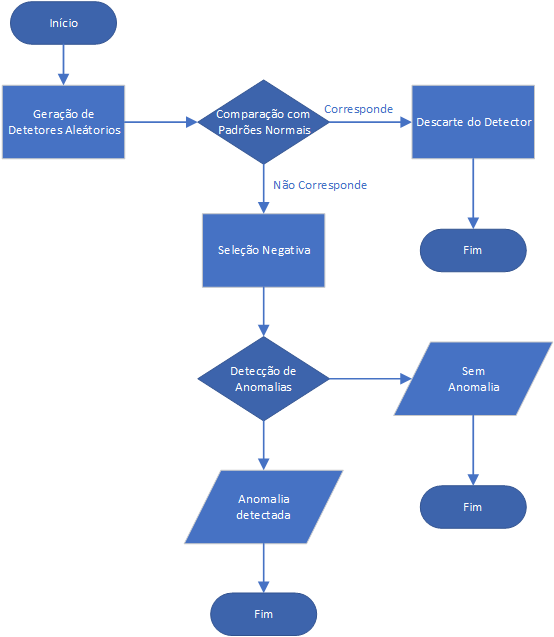
\includegraphics[width=0.65\textwidth]{imgs/algoritmo_selecao_negativa.png}
\caption{Fluxograma do Algoritmo de Seleção Negativa}
\label{fig:fluxograma_selecao_negativa}
Fonte: Autoria própria.
\end{figure}

\chapter{\MakeUppercase{optAiNet}} \thispagestyle{mystyle}

O optAiNet (\textit{Artificial Immune Network for Optimization}) é um algoritmo de otimização inspirado no sistema imunológico que utiliza a abordagem de rede imune artificial (aiNet) para resolver problemas de otimização. A ideia central do optAiNet é a criação de uma população de anticorpos que evolui através de processos de clonagem, mutação e seleção, semelhante ao que ocorre no sistema imunológico natural \cite{optainet2015}.

Além disso, o optAiNet é uma rede artificial que imita o sistema imunológico e é projetada para otimizar funções com variáveis reais. A rede combina os conceitos de seleção clonal e maturação de afinidade com a ideia de uma rede imunológica, proporcionando um equilíbrio sofisticado entre a exploração e a explotação do espaço de busca. Isso abre novas possibilidades em domínios com múltiplos modos.

A optAiNet integra o conceito de rede imunológica através da implementação de um controle dinâmico do tamanho da população. Este controle é responsável por suprimir anticorpos semelhantes e introduzir novos anticorpos, mantendo assim a diversidade da população e permitindo uma exploração adequada do espaço de busca.

Semelhante às técnicas de \textbf{\textit{niching}}\footnote{\textbf{Técnicas de \textit{niching}} são métodos que estendem os algoritmos evolutivos para domínios que requerem a identificação e a manutenção de múltiplas soluções. Inspirados no conceito de nichos ecológicos, que representam regiões do ambiente que suportam diferentes tipos de vida compartilhando os recursos disponíveis, esses métodos foram desenvolvidos com o propósito de manter a diversidade na população e permitir a investigação de múltiplos ótimos de modo paralelo \cite{niching2024}.}, a similaridade entre indivíduos na optAiNet é determinada por uma métrica de distância: dois indivíduos são considerados semelhantes se a distância entre eles for menor que um \textbf{limiar de similaridade}, $\sigma_s$\footnote{O \textbf{limiar de similaridade}, denotado por $\sigma_s$, é um valor que determina o grau de semelhança entre dois indivíduos ou entidades. Se a distância entre dois indivíduos for menor que σs, eles são considerados similares. Este conceito é usado em várias técnicas de niching e algoritmos de otimização, como o optAiNet, para manter a diversidade na população e permitir uma exploração adequada do espaço de busca \cite{limiarizacao2024}}.

Uma característica única da optAiNet é que as operações de supressão e inserção de anticorpos só ocorrem quando se detecta estagnação na população. A estagnação é considerada quando a variação percentual do \textbf{\textit{fitness}} médio da população entre duas iterações é menor que um valor pequeno. Vale ressaltar que essa verificação ocorre apenas em períodos específicos de iterações. Isso permite que a população evolua por um período, através de operações contínuas de seleção clonal e mutação de afinidade, antes de executar a operação de supressão.

\begin{figure}[h]
\centering
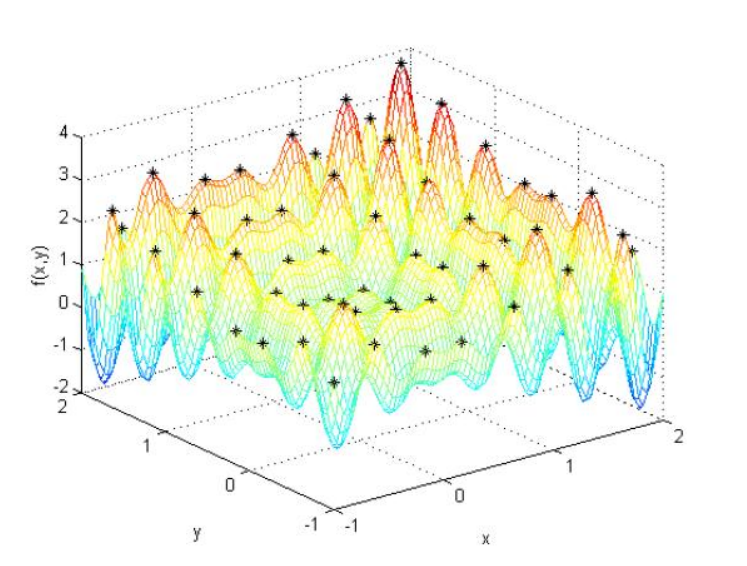
\includegraphics[width=0.8\textwidth]{imgs/populacao_optainet.png}
\caption{Composição da população final após uma execução da optAiNet.}
\label{fig:populacao_optainet}
Fonte: \cite{boccato2024}.
\end{figure}

\section{Como o optAiNet é usado nos SIA} \thispagestyle{mystyle}

Nos Sistemas Imunológicos Artificiais (SIA), o optAiNet é usado para resolver problemas de otimização complexos. Ele gera uma população de soluções (anticorpos) que evolui ao longo do tempo para encontrar a melhor solução possível para o problema em questão.

\subsection{Aplicações e exemplos do optAiNet} \thispagestyle{mystyle}

\begin{itemize}
    \item \textbf{Reconfiguração de Sistemas de Distribuição de Energia Elétrica}: O optAiNet foi aplicado para resolver o problema de reconfiguração de sistemas de distribuição com demandas variáveis não uniformes. O objetivo era encontrar uma única topologia radial que satisfaça os requisitos para operar em todos os níveis de demanda em um sistema de distribuição, visando minimizar os custos de perdas de energia ao longo de um período de operação \cite{optainet2015}.
    
    \item \textbf{Problema do Caixeiro Viajante}: O optAiNet pode ser aplicado para resolver o Problema do Caixeiro Viajante (PCV)\footnote{O \textbf{Problema do Caixeiro Viajante} (PCV) é um problema clássico de otimização combinatória. Ele tenta determinar a menor rota para percorrer uma série de cidades (visitando cada uma delas apenas uma vez), retornando à cidade de origem \cite{matufrgs2024}.}. Neste contexto, cada anticorpo na população representa uma possível rota que visita todas as cidades uma vez e retorna à cidade de origem. O optAiNet pode encontrar a rota mais curta, ou seja, a solução ótima para o PCV, através de um processo iterativo de clonagem, mutação, seleção, e supressão de anticorpos \cite{pvc2011}.
\end{itemize}

\subsection{Fluxograma de um Algoritmo optAiNet} \thispagestyle{mystyle}

\begin{itemize}
    \item \textbf{Geração de população inicial de anticorpos}: Uma população inicial de anticorpos é gerada aleatoriamente.
    
    \item \textbf{Avaliação do \textit{fitness} dos anticorpos}: O \textbf{\textit{fitness}}\footnote{Em um contexto biológico ou de otimização, \textbf{\textit{fitness}} pode se referir à aptidão ou capacidade de um organismo ou solução para sobreviver e se reproduzir no seu meio, ou para atingir um objetivo específico \cite{fitness2024}.} de cada anticorpo na população é avaliado.
    
    \item \textbf{Clonagem dos anticorpos e maturação de afinidade}: Cada anticorpo é clonado e os clones passam por um processo de maturação de afinidade (mutação).
    
    \item \textbf{Seleção dos melhores anticorpos}: Os melhores anticorpos são selecionados com base em seu \textbf{\textit{fitness}}.
    
    \item \textbf{Verificação de estagnação da população}: Verifica-se se a população está estagnada, ou seja, se não houve melhoria significativa no \textbf{\textit{fitness}} médio da população.
    
    \item \textbf{Supressão de anticorpos similares e inserção de novos anticorpos}: Se a população estiver estagnada, os anticorpos que são muito semelhantes entre si são suprimidos e novos anticorpos são inseridos na população.
    
    \item \textbf{Verificação de critério de parada}: Verifica-se se um critério de parada foi atingido. Se sim, o algoritmo termina. Se não, o algoritmo volta para a etapa de clonagem dos anticorpos.
    
    \item \textbf{Fim}: O algoritmo termina e retorna a melhor solução encontrada.
\end{itemize}

\newpage
\thispagestyle{mystyle}

\begin{figure}[H]
\centering
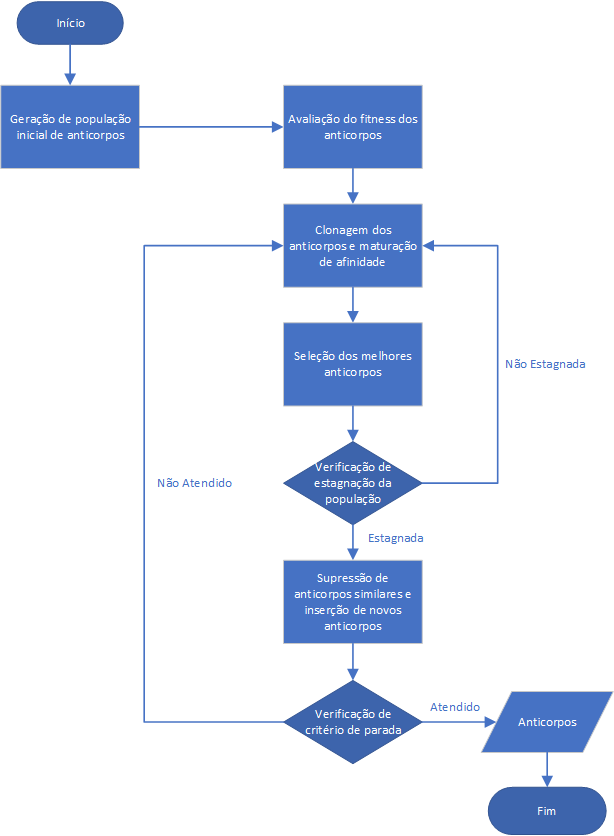
\includegraphics[width=0.8\textwidth]{imgs/algoritmo_optainet.png}
\caption{Fluxograma do Algoritmo de optAiNet.}
\label{fig:fluxograma_optainet}
Fonte: Autoria própria.
\end{figure}

\chapter{\MakeUppercase{Comparação entre Seleção Negativa e optAiNet}}
\thispagestyle{mystyle}

Ambos os algoritmos possuem características e aplicações distintas, sendo importante entender suas diferenças para escolher a ferramenta mais adequada para cada problema.

\subsection{Pontos em comum}

\begin{itemize}
    \item \textbf{Inspiração no sistema imunológico}: Tanto o Algoritmo de Seleção Negativa quanto o optAiNet se baseiam em princípios do sistema imunológico natural para o desenvolvimento de suas funcionalidades. Essa inspiração permite que os algoritmos explorem mecanismos de aprendizagem, memória e adaptação, características essenciais para a resolução de problemas desafiadores.
    
    \item \textbf{Aplicações em SIA}: Ambos os algoritmos encontram aplicações em diversas áreas dentro dos SIA, como detecção de anomalias, otimização e reconhecimento de padrões. A escolha entre um ou outro depende das características específicas do problema a ser resolvido.
\end{itemize}

\subsection{Diferenças}

Diferenças no objetivo:

\begin{itemize}
    \item \textbf{Algoritmo de Seleção Negativa}: O objetivo principal do Algoritmo de Seleção Negativa é identificar anomalias ou intrusões em dados. Ele busca detectar elementos que não se encaixam nos padrões normais, utilizando a analogia da seleção dos \textbf{linfócitos T} no sistema imunológico para combater patógenos.
    
    \item \textbf{optAiNet}: O objetivo principal do optAiNet é resolver problemas de otimização complexos. Ele busca encontrar a melhor solução possível para um problema específico, utilizando a analogia da evolução dos anticorpos no sistema imunológico para encontrar a resposta mais eficaz contra um agente infeccioso.
\end{itemize}

\noindent Diferenças no funcionamento:

\begin{itemize}
    \item \textbf{Algoritmo de Seleção Negativa}: O algoritmo gera um conjunto de detectores aleatórios e os compara com padrões normais. Os detectores que não correspondem a nenhum padrão normal são selecionados e utilizados para identificar novas anomalias.

    \item \textbf{optAiNet}: O algoritmo gera uma população inicial de soluções (anticorpos) e as avalia de acordo com seu \textbf{\textit{fitness}}. As melhores soluções são clonadas e passam por um processo de mutação (maturação de afinidade). As soluções mais aptas são selecionadas, e a população é periodicamente verificada quanto à estagnação. Se estagnada, anticorpos similares são suprimidos e novos anticorpos são inseridos.
\end{itemize}

\subsection{Aplicações específicas} \thispagestyle{mystyle}

\textbf{Algoritmo de Seleção Negativa}:

\begin{itemize}
    \item Detecção de fraudes em transações financeiras;

    \item Detecção de intrusões em redes de computadores;

    \item Detecção de falhas em sistemas de engenharia;

    \item Monitoramento de saúde e diagnóstico de doenças.
\end{itemize}

\noindent \textbf{optAiNet}:

\begin{itemize}
    \item Otimização de rotas de entrega;

    \item Otimização de alocação de recursos;

    \item Otimização de parâmetros de modelos de aprendizado de máquina;

    \item Otimização de \textit{design} de produtos e sistemas.
\end{itemize}

\chapter{Vantagens e Desvantagens} \thispagestyle{mystyle}

\subsection{Algoritmo de Seleção Negativa}

\textbf{Vantagens:}

\begin{itemize}
    \item Eficaz na detecção de anomalias em dados complexos e ruidosos;
    
    \item Simples de implementar e interpretar;

    \item Robusto a \textbf{\textit{outliers}}\footnote{\textbf{\textit{Outliers}}, também conhecidos como valores aberrantes, valores atípicos ou discrepantes, são observações em um conjunto de dados que se desviam significativamente do padrão geral \cite{outliers2023}.}.
\end{itemize}

\noindent \textbf{Desvantagens:}

\begin{itemize}
    \item Pode não ser eficaz na detecção de anomalias sutis;
    
    \item Não otimizado para problemas de otimização;

    \item Requer um conjunto de dados de treinamento com padrões normais.
\end{itemize}

\subsection{optAiNet}

\textbf{Vantagens:}

\begin{itemize}
    \item Eficaz na resolução de problemas de otimização complexos;
    
    \item Capaz de encontrar soluções de alta qualidade;

    \item Robusto a diferentes tipos de problemas;
\end{itemize}

\noindent \textbf{Desvantagens:}

\begin{itemize}
    \item Pode ser mais complexo de implementar e interpretar do que o Algoritmo de Seleção Negativa;
    
    \item Sensível à escolha dos parâmetros do algoritmo;

    \item Pode não ser eficaz em todos os tipos de problemas de otimização.
\end{itemize}
